\section{Modélisation}

	L'analyse préalable nous permet à présent d'avoir une vision plus précise des fonctionnalités de notre programme en vue de réaliser son diagramme de classe. Pour simplifier la modélisation et permettre une plus grande modularité de nos classes nous avons voulu utiliser un maximum de patrons de conceptions. 

	\subsection{patron de Conception}

		\subsubsection{Monteur : création d'une partie}

				\begin{figure}[h]
		\begin{center}
			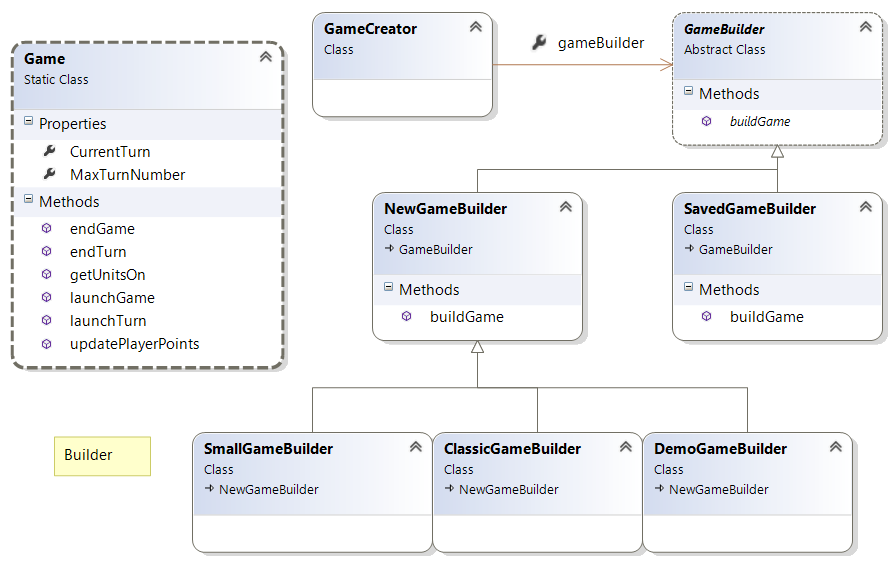
\includegraphics[width=0.8\textwidth]{figure/builder.png}
		\end{center}
		\caption{Création de la partie : patron de conception Monteur}
		\label{fig:builder}
	\end{figure}

		\textbf{Bedbihan} permet aux joueurs de jouer différentes type de parties. Ainsi il existe différentes manières de construire une partie en fonction du type désiré. Néanmoins ces créations passent par des étapes similaires : création de la carte, créations des unités, etc. C'est pourquoi sur  la création de la partie est assurée par le patron de conception \textbf{Monteur}. Ce patron de conception nous permet de séparer la conception de l'objet \emph{Game} de sa représentation. Comme indiqué sur la \textsc{figure} \ref{fig:builder}, la création de la partie sera dirigé par le \emph{GameCreator} qui utilisera le monteur adéquat en fonction de la situation. Ainsi d'une part on minimise le code en évitant des répétitions et de l'autre on gagne en flexibilité : il sera facile de créer un type de partie différent. 



		\subsubsection{Fabrique : création de différents peuples}

		\begin{figure}[h]
			\begin{center}
				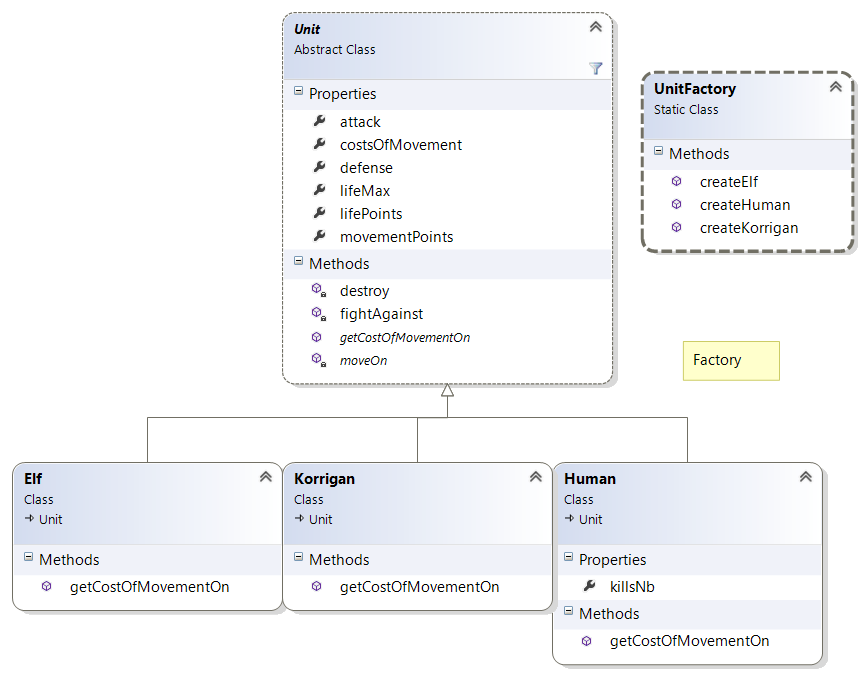
\includegraphics[width=0.8\textwidth]{figure/factory.png}
			\end{center}
			\caption{Création des unités : patron de conception Factory}
			\label{fig:factory}
		\end{figure}

		Chaque joueur possède une armée composé d'un certain nombre d'unités d'un même peuple. Ces unités sont soit des Elfes, des Humains ou des Korrigans. Cette règle se traduis dans notre modélisation, par l'implémentation d'un objet \emph{Player} qui possède une \emph{Faction}, elle même composé d'objets \emph{Units}. Cette modélisation est illustrée par la \textsc{figure} \ref{fig:factory}. \emph{Units} est une classe abstraite implémentée par trois classes concrètes représentants les trois type d'unités disponible. La création de ces unité est assurée par le patron de conception \textbf{Fabrique}. Ce patron de conception nous permettra de créer l'armée adéquate en fonction du peuple choisie par le joueur au lancement de la partie. Il assure une modularité du code, car sa fonction \emph{CreateUnit} retourne un type abstrait. Ainsi, l'appelant n'as pas besoin de se préoccuper de la classe concrète de l'objet retourné par cette méthode. 


		\subsubsection{Poids-mouche : gestion des cases}

		la classe \emph{Game} possède un plateau \emph{Board}. Celui-ci est composé de case \emph{Hexagone}. Or un plateau de type normale contient 225 cases. Ceci impliquerais donc une forte consommation mémoire si chacune de ses cases devait exister en mémoire. C'est pourquoi nous utilisons ici le patron de conception \textbf{Poids-mouche} représenté sur la \textsc{figure} \ref{fig:flyweight}. La classe \emph{HexagonFactory} se charge de fournir les hexagones lors de la création de la carte. Ainsi, lorsqu'il s'agit d'un type de case qui n'a pas encore été instancié il la fabrique, sinon il fournie l'objet préalablement instancié. De cette manière, on représente un nombre importants de cases par la répétitions de quatre cases : \emph{Woods, Mountains, Desert} et \emph{Plain}. Cette modélisation nous impose de ne pas implémenter de paramètres à l'objet \emph{Hexagone} car il serait similaire à toutes les cases de même type. Ainsi, ce seront les objets \emph{Units} qui connaitrons leur position sur le plateau. Les \emph{Hexagones} ne pouvant pas savoir quelles \emph{Units} ils contiennent.

		\begin{figure}
			\begin{center}
				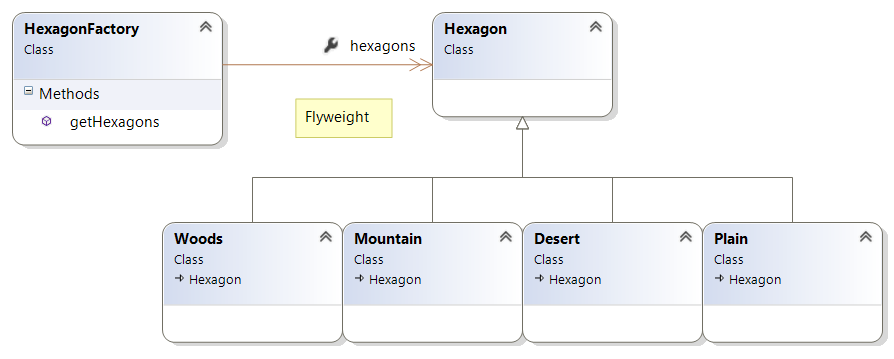
\includegraphics[width=0.8\textwidth]{figure/flyweight.png}
			\end{center}
			\caption{Gestion des cases : patron de conception Poids-mouche}
			\label{fig:flyweight}
		\end{figure}


		\subsubsection{Stratégie : création des différents type de carte}


		\begin{figure}
			\begin{center}
				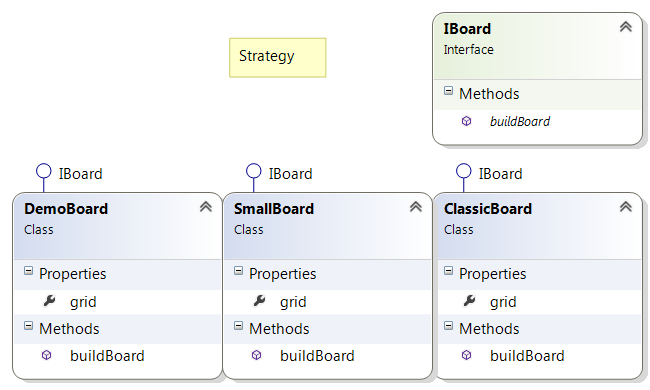
\includegraphics[width=0.7\textwidth]{figure/strategy.png}
			\end{center}
			\caption{Création des différents type de carte : patron de conception stratégie }
			\label{fig:strategy}
		\end{figure}

		Comme dit précédemment, il existe différentes types de cartes : démo, petite et normale. Les tailles sont donc fixé lors de la création de la partie. De plus, le nombre de case d'un même type, Woods, Mountain, Desert ou Plain, doivent être égaux pour assurer l'égalité entre les différents peuples. Par contre, la disposition de ces cases sur le plateau est décidé aléatoirement lors de la création de la partie. Dans un soucis de flexibilité, il est intéressant de pouvoir changer facilement d'algorithme pour construire le plateau. Nous allons donc utiliser le patron de conception \textbf{Stratégie}. Comme le montre la \textsc{figure} \ref{fig:strategy} La classe \emph{Board} possède un paramètre \emph{StrategyBoard} interchangeable qui définit la stratégie d'implémentation du plateau. 

	\subsection{Diagramme de classe}


	\begin{figure}
		\begin{center}
			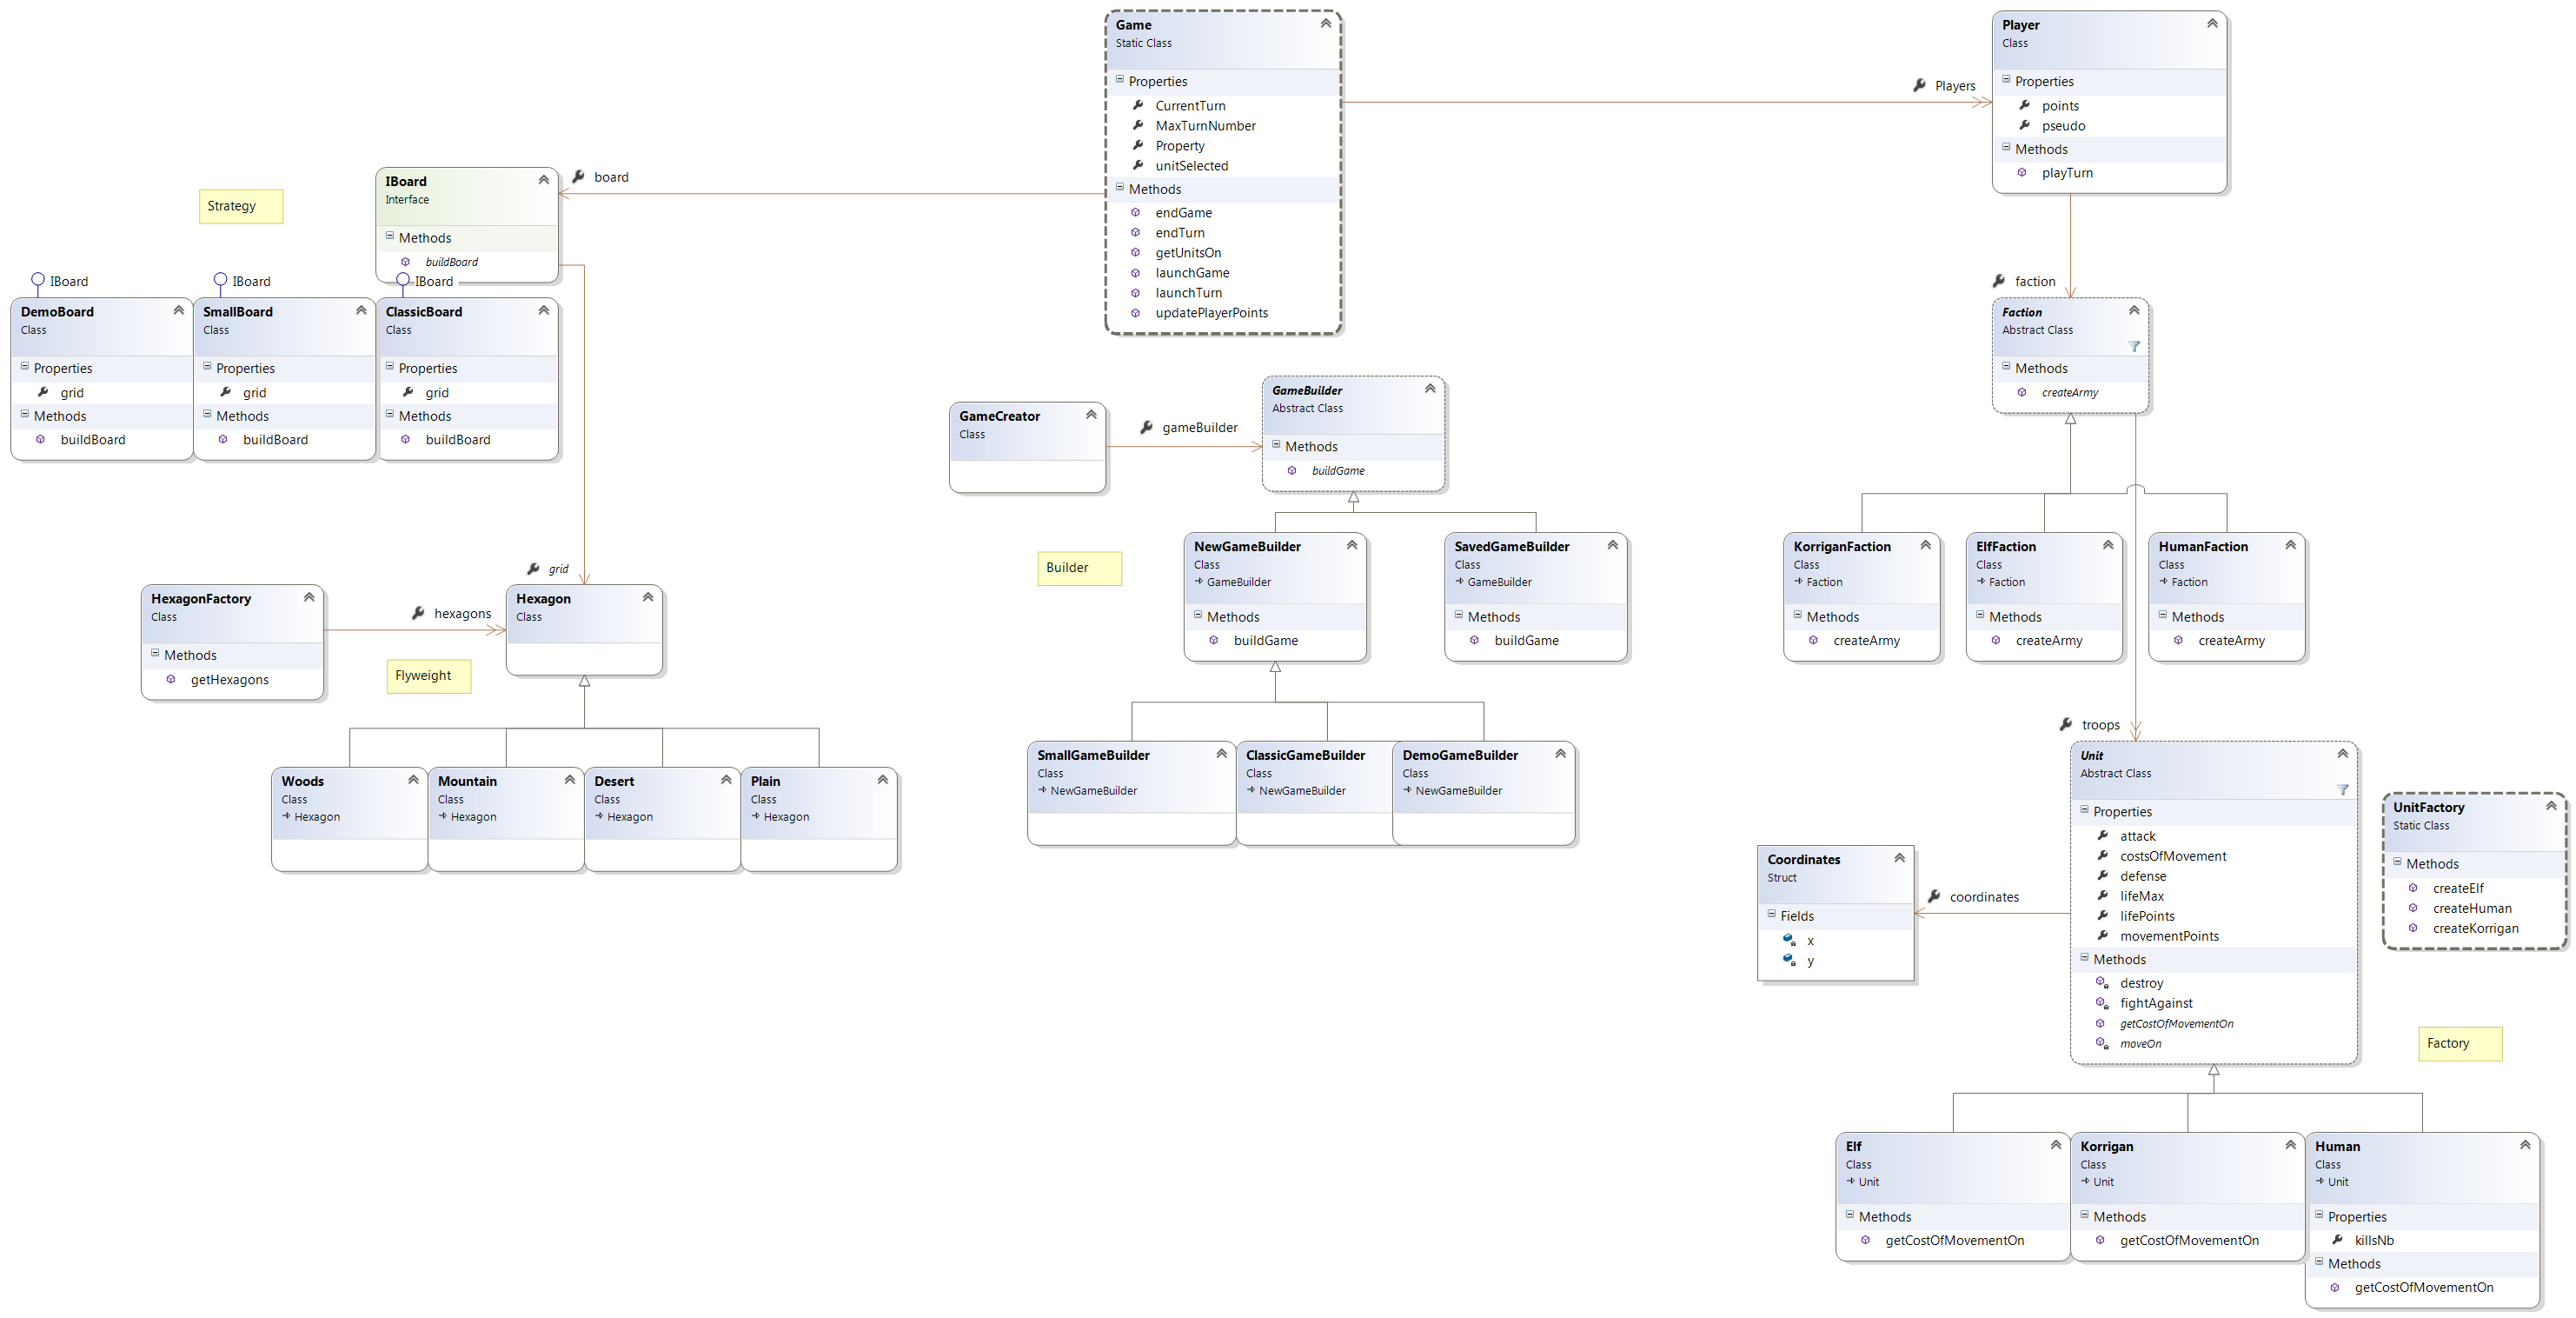
\includegraphics[width=0.5\textwidth]{figure/entire_class_diagram}
		\end{center}
		\caption{Diagramme de classe}
		\label{fig:class_global}
	\end{figure}




